In this chapter, we will focus our attention on Redis. Redis is officially described as ``in-memory data structure store, used as database, cache and message broker.'' \cite{sanfilippo2009redis} Like Memcached, Redis provides a simple text based API with \textit{get}, \textit{set}, and many more advanced features, for interaction over the network. Unlike Memcached, Redis is single threaded by design which introduces interesting scalability challenges.

We initially focus on the default performance of Redis when it is first deployed. Subsequently, we will turn our attention to Redis scalability as well as performance under various scenarios. We will consider the effect of multiple Redis instances, process pinning and IRQ Affinity. Furthermore we will explore Redis performance with different object sizes and key distributions.

Throughout this chapter, we focus on key performance metrics - throughput, mean and tail (99th) percentile latency as well as the target Quality of Service (QoS) of 99th percentile latency within 1 millisecond. Unless otherwise stated, all benchmarks are performed to target the QoS.


\section{Out of the Box Performance}
Firstly, we focus on the default Redis performance. Redis comes with a configuration file \texttt{redis.conf}\cite{RedisConfiguration} with sensible defaults. Redis supports data persistence management and by default keys are not evicted when the cache fills up. For the purposes of this paper, we are interested an eviction based cache and as such will configure Redis to use the Least Recently Used policy for key replacement. Configuration options can be supplied on the command line as well and override any configuration options specified in \texttt{redis.conf}. Table \ref{tab:r_redis_baseline_config} summarizes our default Redis configuration.

\begin{table}[h!]
\centering
\begin{tabular}{| c c c |}
 \hline
 Configuration Option & Explanation & Value\\ [0.5ex]
 \hline\hline

 --port & Port number & 11120 \\
 --maxmemory & Maximum used memory & 6GB \\
 --maxmemory-policy & Policy for key evictions & allkeys-lru \\

 \hline

\end{tabular}
\caption{Redis Configuration}
\label{tab:r_redis_baseline_config}
\end{table}

With the configuration defined, we can deploy the Redis application with the following command.

\begin{lstlisting}
redis redis.conf --port 11120 --maxmemory=6GB
    --maxmemory-policy=allkeys-lru
\end{lstlisting}

In order to get an initial feel for Redis performance, we setup the benchmark to increase load on the cache server linearly. Table \ref{tab:r_memtier_baseline_config} outlines the configuration used for the Memtier benchmark.

\begin{table}[h!]
\centering
\begin{tabular}{| c c c |}
 \hline
 Configuration Option & Explanation & Value\\ [0.5ex]
 \hline\hline

 -s & Server & nsl200 (server hostname) \\
 -p & Port number & 11120 \\
 -c & Number of Connections & [1..10] \\
 -t & Number of Threads & 2 \\
 --key-minimum & Smallest key & 1 \\
 --key-maximum & Largest key & 100 000 000 \\
 --random-data & Generate Random Data & true \\
 --data-size & The size of data in bytes & 64 \\

 \hline

\end{tabular}
\caption{Memtier Configuration Options}
\label{tab:r_memtier_baseline_config}
\end{table}

Memtier can be started with the following command:
\begin{lstlisting}
  memtier -s <server> -p 11120 -c <connections> -t 2
    --random-data
    --key-minimum=1
    --key-maximum=100000000
    --random-data
    --data-size=64
\end{lstlisting}

We are showing the Redis deployment command as well as the Memtier command here for clarity, however, the commands will be omitted in subsequent sections.

\subsection{Latency \& Throughput vs Connections}
\begin{figure}[h]
    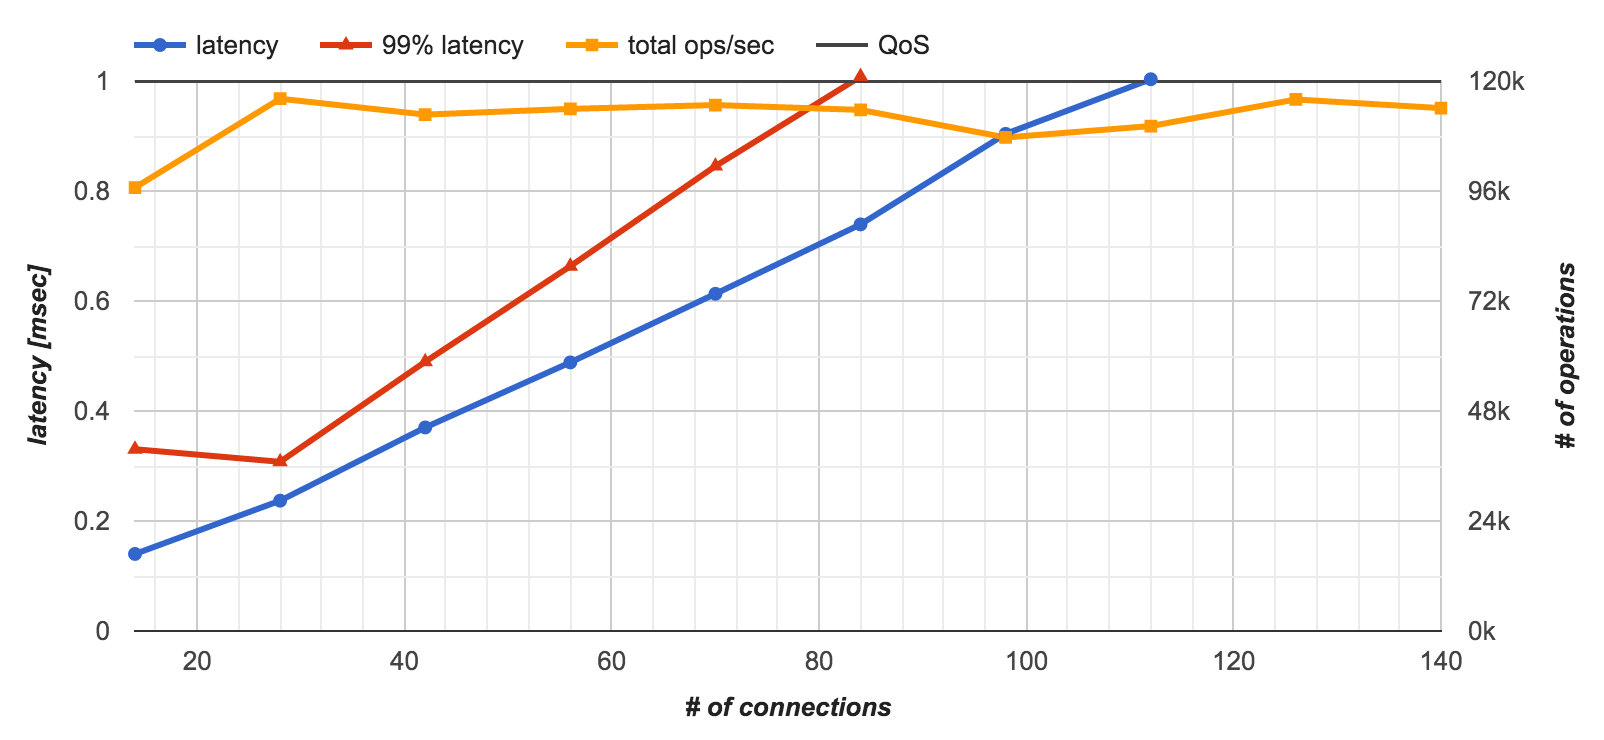
\includegraphics[width=\textwidth]{./res2/r_baseline_latency.png}
    \caption{Latency \& Throughput vs Number of Connections}
    \label{fig:r_baseline_latency}
\end{figure}

Figure \ref{fig:r_baseline_latency} plots the relationship between mean latency, 99th percentile latency and the number of operations per second against the number of connections.
The mean latency increases with the number of connections linearly. Similarly, the 99th percentile latency increases linearly as the number of connections increases, however, it grows faster than the man latency. At 56 connections, we obtain a 99th percentile latency of 0.88 ms. A further increase in the number of connections leads to QoS violation.
The number of operations per second remains constant with the number of connections and latency within QoS. The cache executes 93k requests per second, however, at this load we are unable to increase throughput while satisfying our QoS.

\subsection{CPU Utilization}
\begin{figure}[h]
    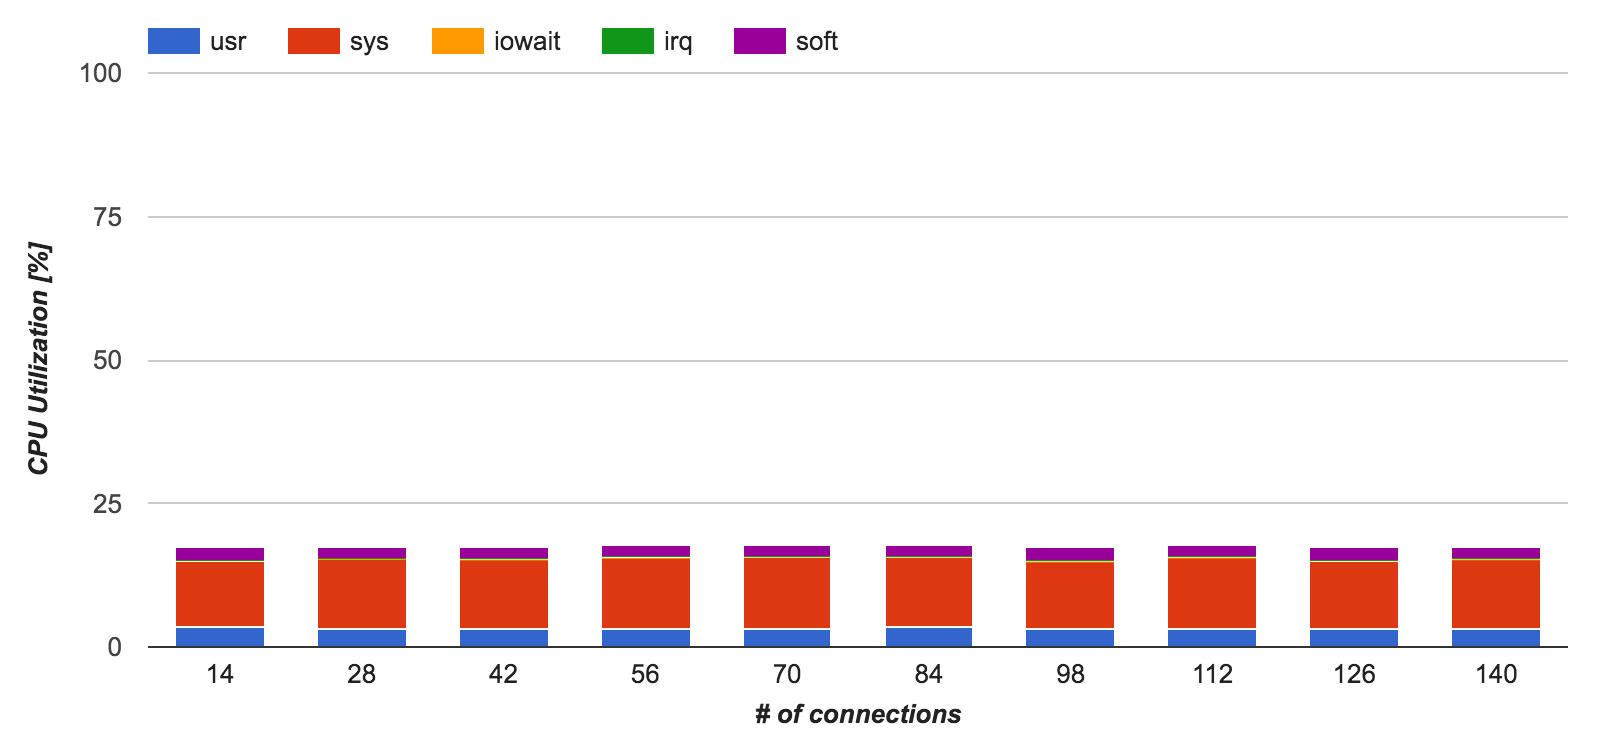
\includegraphics[width=\textwidth]{./res2/r_baseline_cpu.png}
    \caption{Default Redis CPU Utilization vs Number of Connections}
    \label{fig:r_baseline_cpu}
\end{figure}

Figure \ref{fig:r_baseline_cpu} plots the relationship between CPU utilization as reported by \textit{mpstat} and the number of connections. Firstly, we can observe that the total utilization remains stable at 17\%. We can clearly see that overall the server is heavily underutilized. However, the aggregate breakdown across all CPUs is misleading in this case. Figure \ref{fig:r_baseline_cpu_individual} shows the individual CPU utilization for 56 client connections. We can observe that we achieve nearly 100\% utilization on core 0 while the remaining cores are idle. Furthermore, we can observe that Redis accounts for only 14\% utilization while the rest is used for kernel processing (46\%) and software interrupt processing (34\%). From the breakdown, we can conclude Redis utilization is kernel and software interrupt dominated rather than application processing dominated.

\begin{figure}[h]
    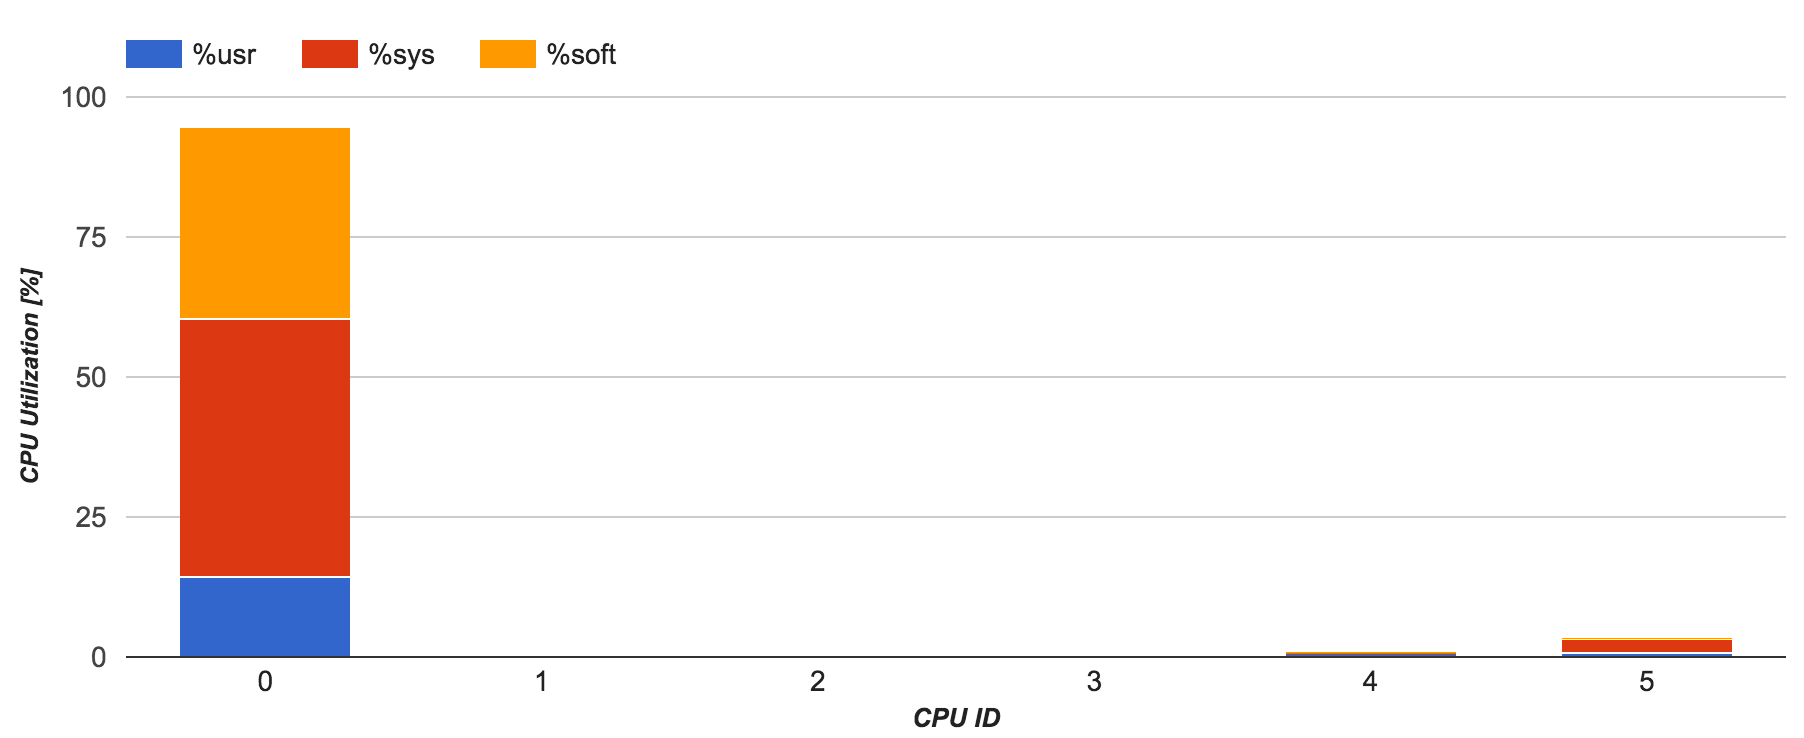
\includegraphics[width=\textwidth]{./res2/r_baseline_cpu_individual.png}
    \caption{Default Redis Individual CPU Utilization at 56 connections}
    \label{fig:r_baseline_cpu_individual}
\end{figure}

\subsection{Conclusion}
We have shown that Redis is capable of delivering 93k requests per second in its default configuration without any optimizations. Additionally, we have observed the impact of single threaded Redis on the overall host CPU utilization as well as the breakdown per individual core. We have also shown that the kernel and software interrupt processing play a significant role in overall performance.


\section{Multiple Redis Instances}
\label{sec:multiple-redis-instances}

As seen in previous section, the overall cache server utilization suffers from single threaded nature of Redis. An immediate solution to this problem is to deploy multiple instances simultaneously. In this section, we consider a multi-instance Redis setup. It is important to keep in mind that each individual instance is completely isolated from the rest. As a result, the amount of memory space available to each instance decreases and therefore the key range we can store on each instance decreases. An application requiring access to a large number of keys will therefore be forced to partition the key space. Client side consistent hashing has the ability to alleviate this problem. Alternatively, a proxy application such as Twemproxy \cite{twemproxy} can be used to spread the load and create a single point of access to the instances.

As the number of instances increases on the server, we expect the overall throughput to increase. As such, we initially utilize a larger number of connections than in the previous section, namely we use 210 connections (30 connections per each benchmarking host). We have determined empirically that 30 connections allow us to demonstrate Redis multi-instance scalability effectively. Additionally, 30 provides a great deal of flexibility when dealing with load partitioning across instances as we have 6 CPU cores available to us on the server. We consider 5 distinct multi-instance scenarios, they breakdown is outlined in Table \ref{tab:redis_instances}.

\begin{table}[h!]
\centering
\begin{tabular}{| c c c c |}
 \hline
 Instance Count & Connections & Threads & Total\\ [0.5ex]
 \hline\hline

 1  & 5 & 6 & 30 \\
 2  & 5 & 3 & 30 \\
 3  & 5 & 2 & 30 \\
 6  & 5 & 1 & 30 \\
 10 & 3 & 1 & 30 \\
 \hline

\end{tabular}
\caption{Multi Instance Scenarios with Memtier connections and thread counts}
\label{tab:redis_instances}
\end{table}

Consequently, we can define the following Redis configuration for each scenario. We maintain the same amount total memory while partitioning it evenly across instances. We of course also use the LRU Redis policy.

\begin{table}[h!]
\centering
\begin{tabular}{| c c c |}
 \hline
 Instances & Memory & Total Memory\\ [0.5ex]
 \hline\hline

 1  & 6GB & 6GB \\
 2  & 3GB & 6GB \\
 3  & 2GB & 6GB \\
 6  &  1GB & 6GB \\
 10 &  0.6GB & 6GB \\
 \hline

\end{tabular}
\caption{Redis Maximum Memory config per number of instances}
\label{tab:redis_instances}
\end{table}


\subsection{Latency \& Throughput vs Instances}
\begin{figure}[h]
    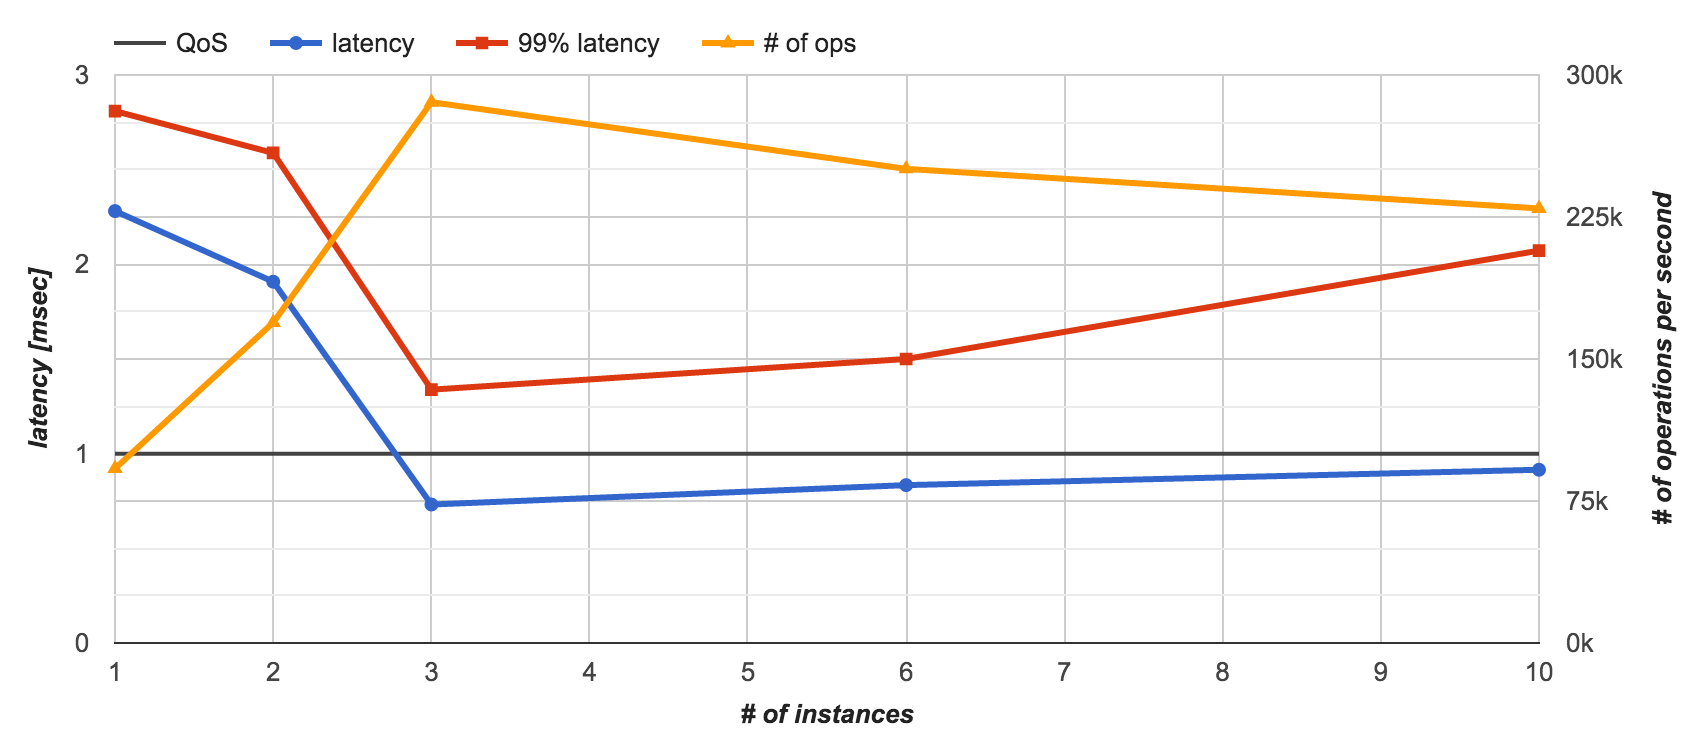
\includegraphics[width=\textwidth]{./res2/r_instances_latency.png}
    \caption{Redis Instances: Latency \& Throughput}
    \label{fig:r_instances_latency}
\end{figure}

Figure \ref{fig:r_instances_latency} plots the relationship between latency, throughput and the number of instances.

Firstly, as the number of instances increases, both 99th and mean latency decrease and a reach a minimum at 3 instances. At 3 instances, we obtain a 99th percentile latency of 1.33 milliseconds, above the requires QoS. As the number of instances increases further, both mean and tail latency increase too.

Secondly, as the number of instances increases, throughput does too up to 3 instances where it reaches a maximum of 285k requests per second. A further increase in the number of instances leads to a decrease in throughput.

We can observe that multiple Redis instances do not scale as expected. We would expect the maximum throughput with the minimum tail latency to be achieved at 6 instances as we have 6 cpu cores. However, we maximize throughput while minimizing tail latency at 3 instances instead. Let us investigate the CPU utilization to get a better insight into the problem.

\subsection{CPU vs Instances}
\begin{figure}[h]
    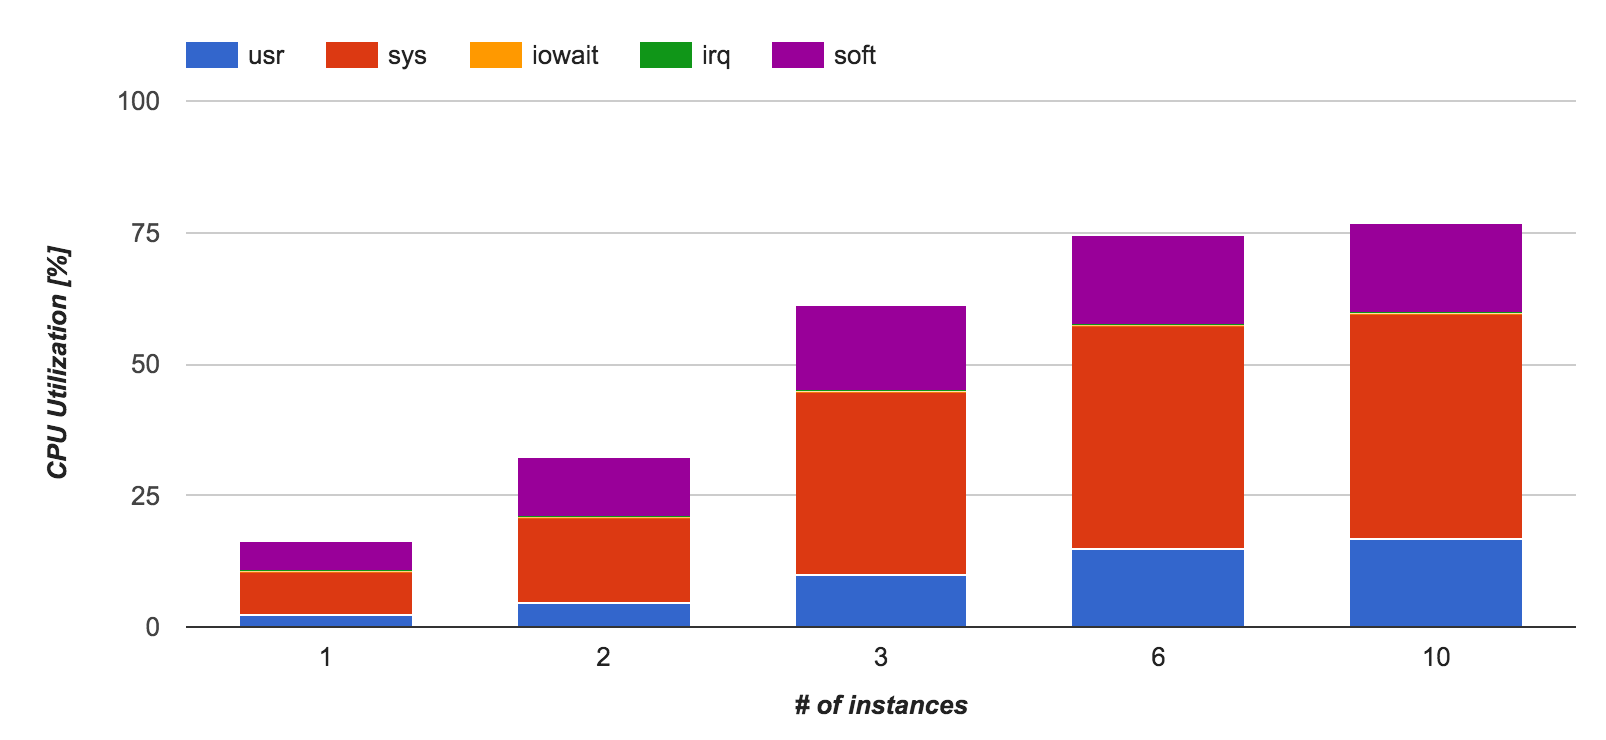
\includegraphics[width=\textwidth]{./res2/r_instances_cpu.png}
    \caption{Redis Instances CPU}
    \label{fig:r_instances_cpu}
\end{figure}

Figure \ref{fig:r_instances_cpu} plots the CPU utilization against the number of instances with the respective category breakdown as reported by \textit{mpstat}. We can observe that as we increase the number of instances, total CPU utilization increases. However, at no point do we reach a 100\% utilization on the server. The utilization remains capped at 75\% for configurations with 6 and 10 instances. Let us investigate the distribution of work on individual cores to get a better insight into the problem.

Figure \ref{fig:r_instances_cpu_individual} outlines the CPU utilization per individual CPU core with 6 instances. We can observe that all software interrupts are processed on core 0 with 100\% utilization while the remaining cores remain underutilized. This renders core 0 a bottleneck for the remaining CPU cores and results in underutilization of resources.

\begin{figure}[h]
    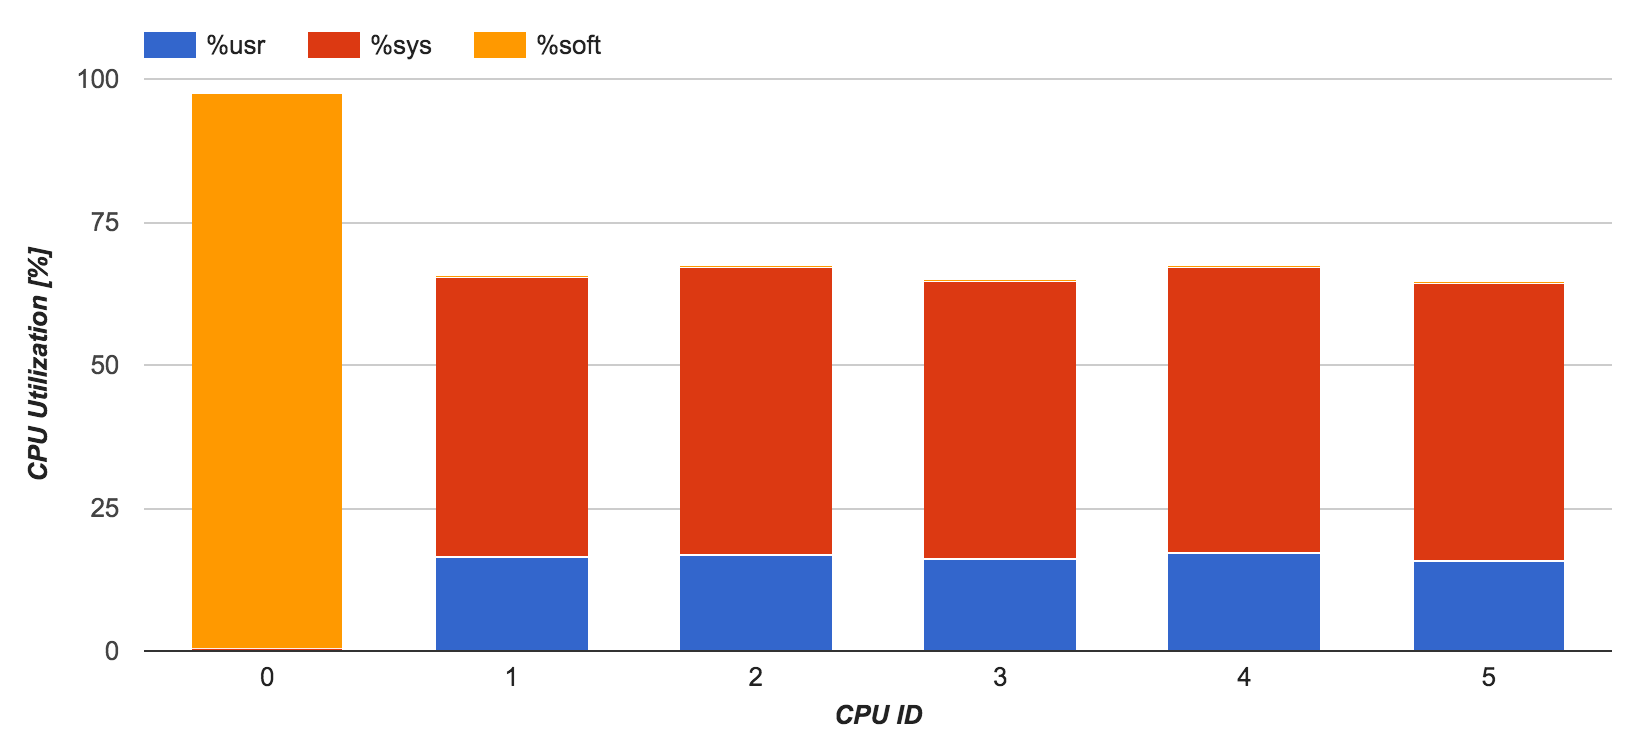
\includegraphics[width=\textwidth]{./res2/r_instances_cpu_individual.png}
    \caption{Redis Instances: Individual CPU Utilization at 6 instances}
    \label{fig:r_instances_cpu_individual}
\end{figure}

\subsection{Multiple Instances Conclusion}
We have shown that multiple Redis instances do not scale linearly with the number of instances. In our benchmark, we have observed that the software interrupt processing is the bottleneck of multiple instances. We will address the load imbalance problem in the following chapter through IRQ Affinity pinning.

% ____________________________________________________
\section{IRQ Affinity}
In this chapter we turn our attention to addressing the load imbalance problem observed in when scaling Redis across multiple instances. In order to spread the software interrupt processing work across to multiple cores, we will assign each individual core a unique CPU core affinity. This process is outlined in detail in Section \ref{sec:m_irq_affinity}.

With IRQ Affinity assigned, we would expect the software interrupt processing to be spread evenly across all CPU cores and therefore removing the single CPU core bottleneck observed in the previous chapter.

\subsection{Latency \& Throughput with IRQ Affinity}
\begin{figure}[h]
    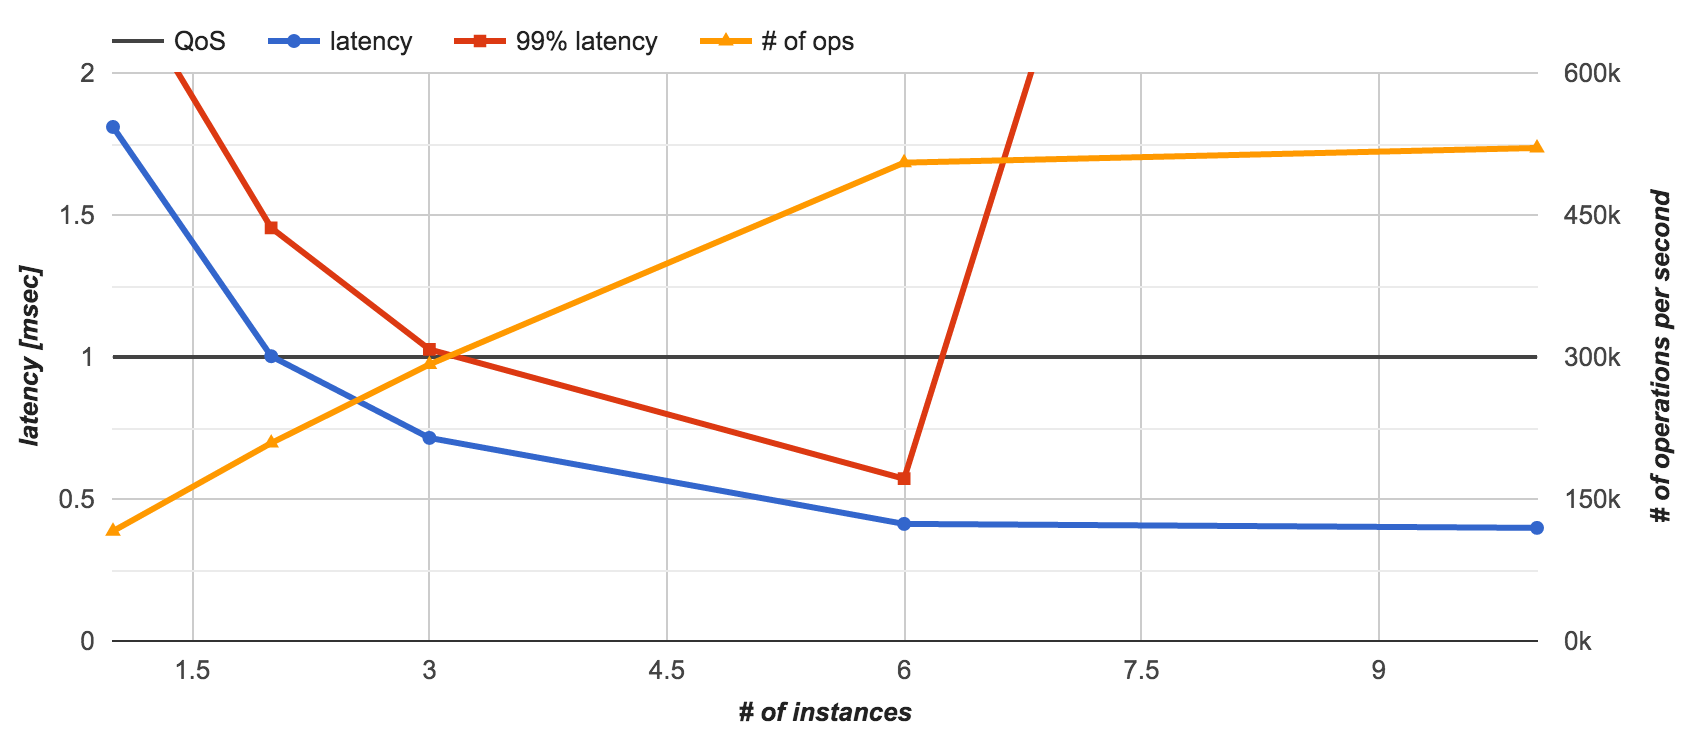
\includegraphics[width=\textwidth]{./res2/r_irq_latency.png}
    \caption{Redis Instances with IRQ Pinned: Latency \& Throughput}
    \label{fig:r_irq_latency}
\end{figure}

Figure \ref{fig:r_irq_latency} plots the relationship between latency, throughput and number of instances after IRQ pinning. Firstly, mean latency decreases as the number of instances increases up until it reaches a minimum of 0.4 ms at 6 instances. A further increase in the number of instances does not affect the mean latency. Secondly, the 99th percentile latency decreases sharply between 1 and 6 instances. It reaches a minimum of 0.57 ms at 6 instances. Additional instances lead to a sharp increase in tail latency. Furthermore, the number of operations increases steadily between 1 and 6 instances. There is a linear relationship between the number of instances and throughput with up to 6 instances. At 6 instances, we obtain 502k requests per second. A further increase in the number of instances leads to a slight increase in the number of operations, however, it is outside of the QoS constraints for tail latency.

\subsection{CPU Utilization with IRQ Affinity}
\begin{figure}[h]
    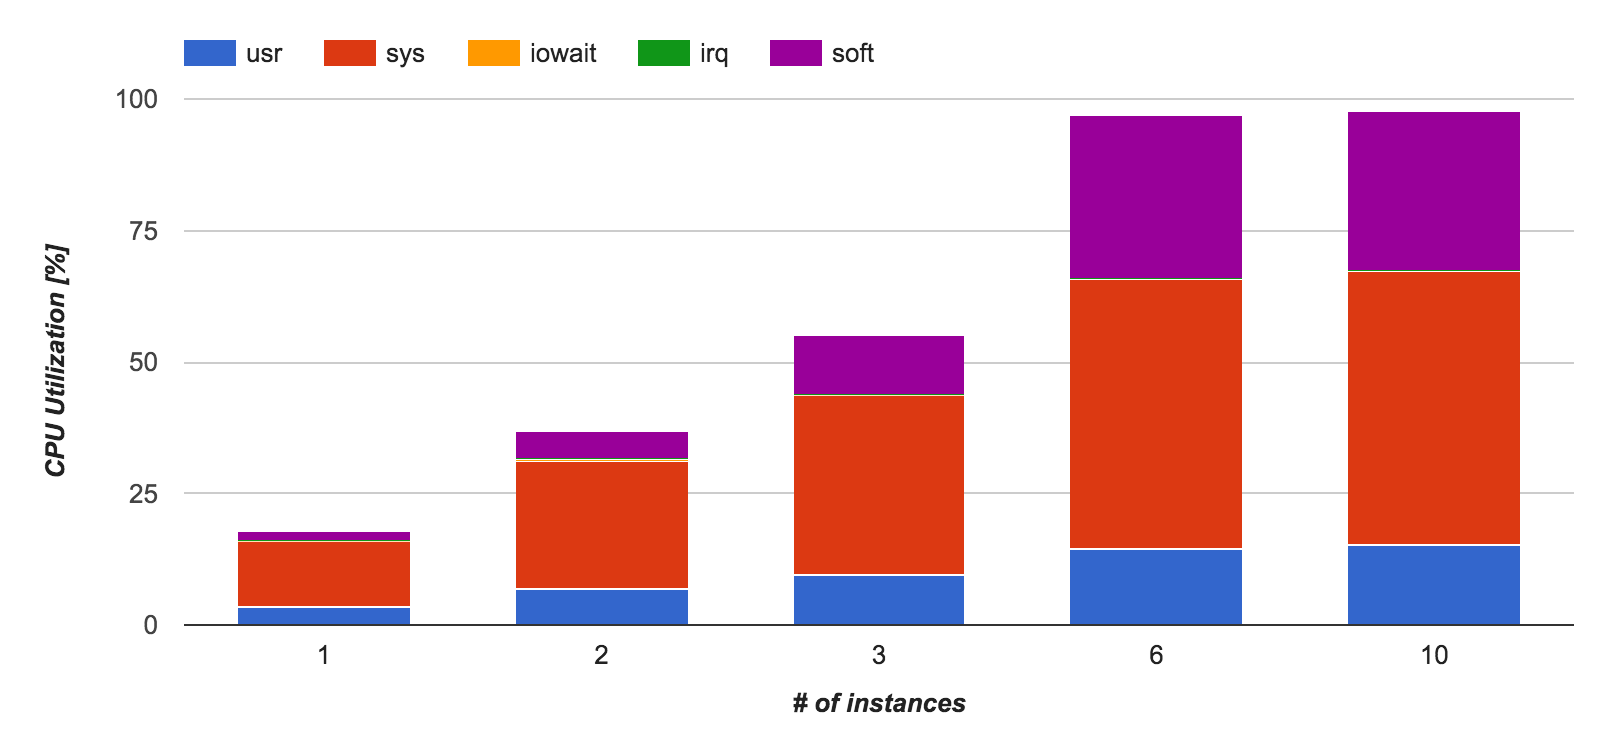
\includegraphics[width=\textwidth]{./res2/r_irq_cpu.png}
    \caption{Redis Instances with IRQ Pinned: CPU Utilization}
    \label{fig:r_irq_cpu}
\end{figure}

Figure \ref{fig:r_irq_cpu} plots the category breakdown of CPU utilization against the number of instances. We can observe that the total utilization is nearly 100\%. Additionally, we can observe that the proportion of kernel, user and software interrupt utilization increases linearly with the number of instances. This is indicative of good multi-instance scalability. At 10 instances, we obtain the same utilization as well as category utilization as with 6 instances. This is due to hard constraint on the amount of resources available on the server.

Inspecting individual CPU core utilization in Figure \ref{fig:r_irq_cpu_individual} at 6 instances, we can observe that software interrupt processing is spread across all CPU cores and allows all cores to be fully utilized.

\begin{figure}[h]
    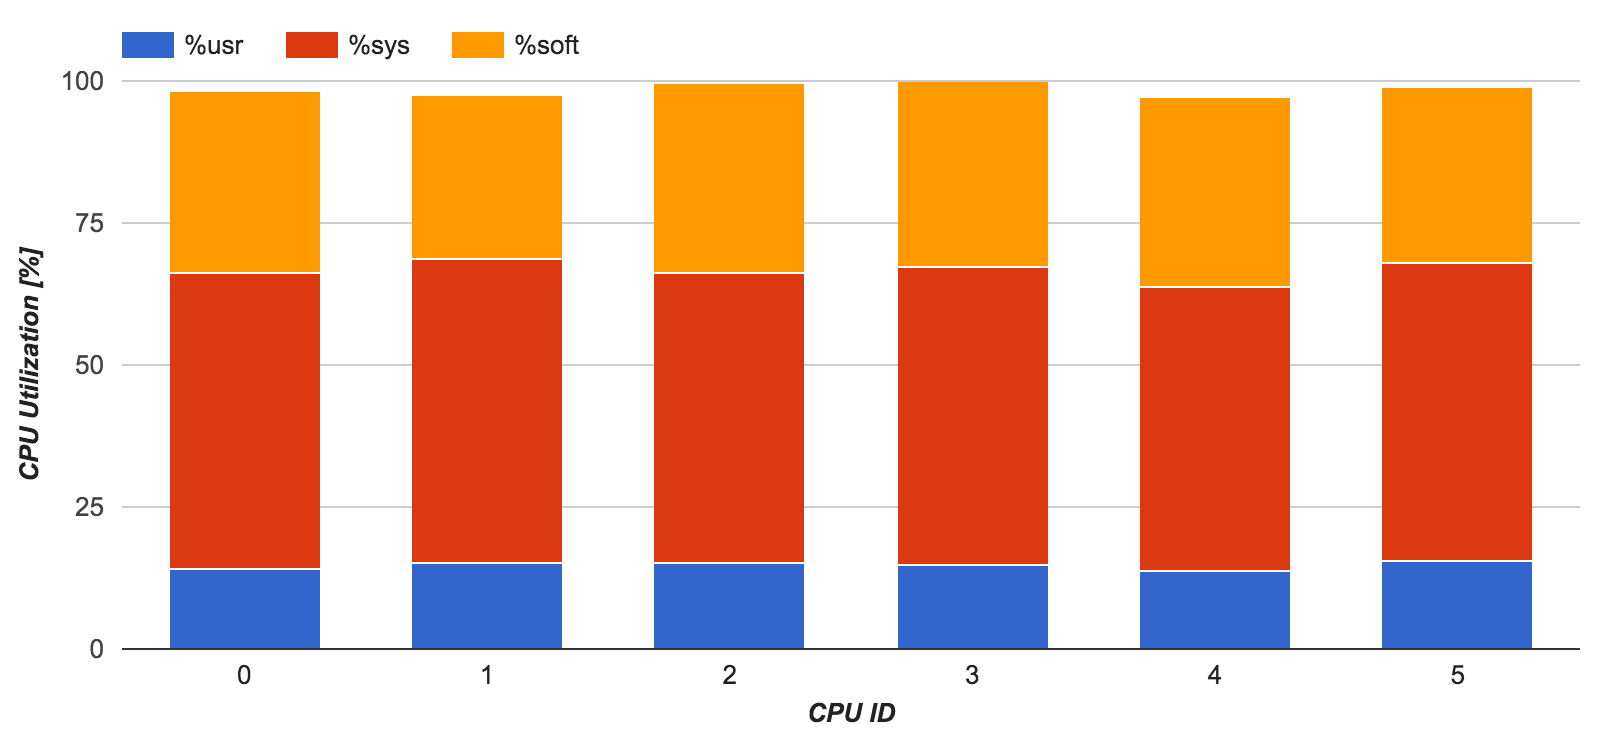
\includegraphics[width=\textwidth]{./res2/r_irq_cpu_individual.png}
    \caption{Redis Instances with IRQ Pinned: Individual CPU utilization at 6 instances}
    \label{fig:r_irq_cpu_individual}
\end{figure}

\subsection{IRQ Affinity Conclusion}
In this section, we have shown that software interrupt processing is essential to good Redis performance. By spreading the software interrupt handling onto multiple CPU cores, we have been able to achieve linear scalability with the number of instances up to the hard limit of the number of CPU cores. This is significantly more than without IRQ pinning. Additionally, we have shown that Redis is capable of delivering 500k requests per second with 6 instances while satisfying QoS constraints. It is worth noting that the tail latency of Redis exhibits relatively small deviation from the mean latency. This suggests that there are only a small number of requests taking above average time to process and further indicates good scalability in terms of multiple instances.


% ____________________________________________________
\section{Pinned Redis Instances}
In this section, we take a brief look at process pinning. Process pinning is an assignment of CPU affinity to a particular process. Similarly to thread pinning, we can pin processes to individual cores. In this benchmark, we consider the best found configuration so far, that is 30 connections with IRQ affinity set.

Firstly, after starting Redis, we can discover the required process IDs through the use of the \textit{ps} utility. Assigning process affinity can then be done through the \textit{taskset} utility. The following bash command sets the CPU affinity of process \textit{pid} to core \textit{5}.

\begin{lstlisting}
  taskset -pc 5 pid
\end{lstlisting}

It has been suggested that process and thread pinning can help reduce ``load imbalance'' \cite{leverich2014reconciling} by reducing interference caused by scheduling multiple simultaneous workloads. However, in our benchmarks we have not been able to obtain any significant speed up by pinning Redis processes to individual cores. We have obtained nearly identical results as with IRQ pinning and for clarity purposes will not be including a figure.

% ____________________________________________________
\section{Object Size}
In this section, we shift our focus from improving the performance of the cache itself to understanding how it performs under various scenarios, namely how does the size of each object stored impact overall performance within the QoS.

We consider the case of increasing the object size by a factor of 2 at each step. We utilize the same configuration for Memtier as in Section \ref{sec:m_object_size}. The generated dataset remains the same in size while the range of possible keys shifts to account for the increased individual object size.

\subsection{Latency \& Throughput vs Object Size}
\begin{figure}[h]
    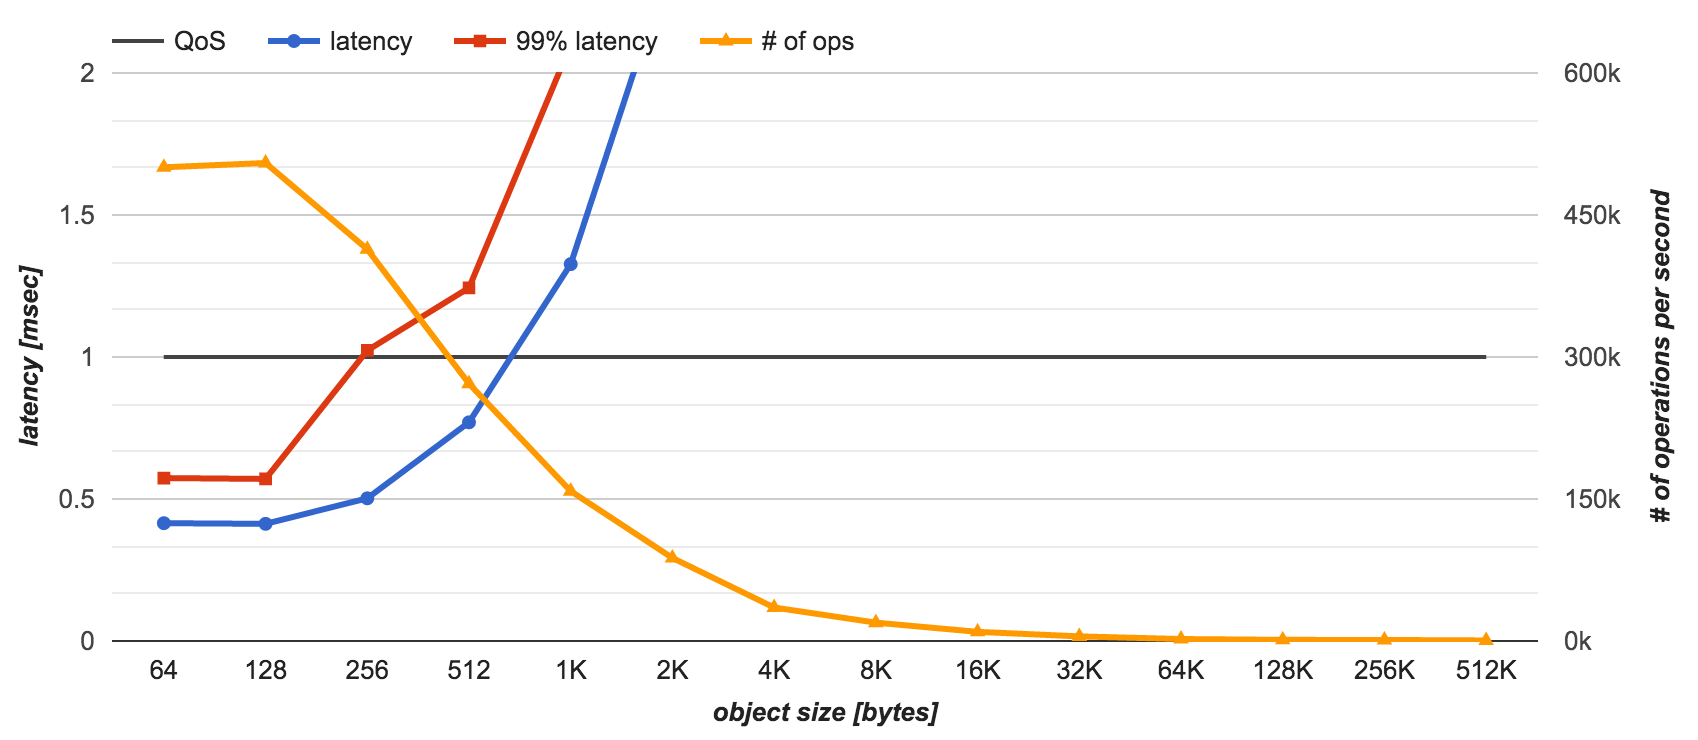
\includegraphics[width=\textwidth]{./res2/r_object_size_latency.png}
    \caption{Redis \& Object size: Latency and Throughput}
    \label{fig:r_object_size_latency}
\end{figure}

Figure \ref{fig:r_object_size_latency} plots the relationship between object size, latency and throughput. Please note that the horizontal axis increases in multiples of 2.

Initially, we start with object size of 64 bytes, the object size used all previous benchmarks. This serves as a baseline. As object size increases to 128, we observe an slight increase in the number of operations. Mean and tail latency remain the same.

Subsequently, as object size grows, we observe a decrease in the total number of operations and an increase in both mean and tail latency. In fact, QoS constraints are already violated with object sizes 256 bytes large. As object size increases even more, throughput falls drastically while mean and tail latency sky rockets.

As object size increases, the pattern of execution becomes network dominated rather than computation dominated. Larger objects take longer to transmit resulting in increased tail latency.

\subsection{Latency \& Throughput vs Object Size}
\begin{figure}[h]
    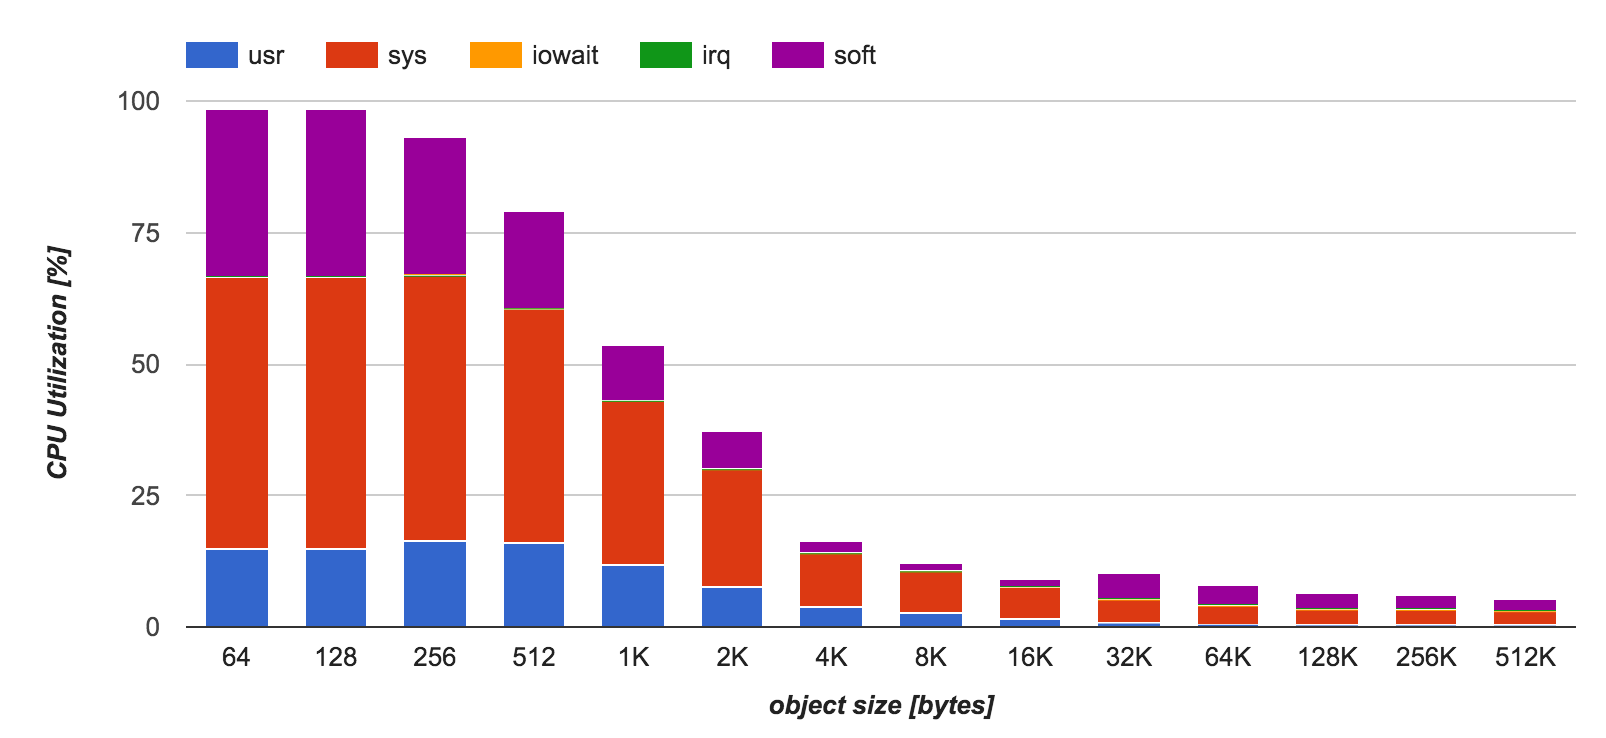
\includegraphics[width=\textwidth]{./res2/r_object_size_cpu.png}
    \caption{Redis \& Object size: CPU Utilization}
    \label{fig:r_object_size_cpu}
\end{figure}

Figure \ref{fig:r_object_size_cpu} considers the effect of object size on the CPU utilization of the server. Initially, we obtain a 100\% utilization on the server side with object sizes 64 and 128 bytes large. As object size increases, and the tail latency increases, the inter-arrival time of each packet also increases. This results in reduced utilization. Effectively, the server is idle awaiting work. This pattern dominates as object size increases further.

\subsection{Object Size Conclusion}


% ____________________________________________________
\section{Key Distributions}
TODO